\newcommand*{\sfas}{\mathfrak s}
\newcommand*{\lfas}{\mathfrak l}
\newcommand*{\gfas}{\mathfrak g}
\newcommand*{\crt}{\mathrm C}

\definecolor{gr1}{gray}{.9}
\definecolor{gr2}{gray}{.8}
\definecolor{gr3}{gray}{.7}
\definecolor{gr4}{gray}{.6}
\definecolor{grmixed}{gray}{.75833}%1-29/120
\definecolor{gclr}{gray}{.95}
\definecolor{lclr}{gray}{.8}
\definecolor{sclr}{gray}{.6}
\definecolor{glclr}{gray}{.875}
\definecolor{lsclr}{gray}{.7}
\definecolor{sgclr}{gray}{.775}

% \setcounter{section}{-1}
\section{热力学基本定律}
%\subsection*{宏观}
宏观物质可以用很少的量表征。这种特性源于\textit{宏观测量与原子时间尺度相比极其缓慢,与原子空间尺度相比十分粗糙。}宏观体系忽略了系统内部每个粒子的具体运动,正如Anderson所说:\textbf{\textit{More is different.}}
而热力学便是\textit{唯象}地描述多粒子行为的宏观理论。

\paragraph*{热力学系统}大量微观粒子(分子、原子、电子等)组成的有限的宏观体系。平衡态:宏观性质不随时间改变的状态。自由度:独立的宏观量数目。
\begin{theorem}{热平衡定律}{Law of Thermal Equilibrium}
	若系统A和系统B平衡,和系统C也平衡,则B和C平衡。
\end{theorem}
因此互为平衡的体系有一共同的物理性质:温度$T$。
\begin{definition}{物态方程}{State Equation}
	$T$与其它状态参量间的关系。比如
	\begin{align}
		\text{理想气体:}&&pV&=nRT.\\
		\text{Van der Waals气体:}&&\kh{p+a\frac{n^2}{V^2}}&(V-nb)=nRT.
	\end{align}
\end{definition}
\paragraph*{准静态过程}%{Quasistatic process}
每一瞬时,状态无限接近平衡态。

系统的能量包括内能$U$和整体运动能量;对于封闭系统的能量交换有功$W$和热量$Q$两种方式。准静态过程中,
\begin{align}
	\vd W=\sum Y_i\d y_i,
\end{align}
$(Y_i,y_i)$分别是广义力和广义坐标,如$(-p,V),(\mu_0H,M),(\sigma,A)$等。
\begin{theorem}{能量守恒定律}{Energy Conservation Law}
	一个热力学系统的内能增量$\d U$等于外界对它所做的功$\vd W$与外界向它传递的热量$\vd Q$的和:
	\begin{align}
		\d U=\vd W+\vd Q.
	\end{align}
\end{theorem}
%关于能量的\textit{可测量性}。由能量守恒,
\indent 如果系统是\textbf{绝热}($\vd Q\equiv 0$)的,我们便可以用机械功$\vd W$测量内能的变化$\D U$,通过指定基准态的内能$U_0$就可以得出任意状态的内能$U$。进而我们可以测量导热系统的传热$\vd Q$。

定义热容量
\[C=\lim_{\D T\to0}\frac{\D Q}{\D T},\]
显然,热容量与过程相关。再定义比热为单位质量的热容量,定容热容量和定压热容量分别为
\begin{align}
	C_V=\kh{\pv UT}_V,\quad C_p=\kh{\pv HT}_p.
\end{align}

内能标准全微分式:将$U$全微分式中各变量微分前的系数用可测量表达出来。
\begin{example}{静流体系统}{Static Fluid System}
	以$T,V$为变量
	\[\d U=\underset{C_V}{\underline{\kh{\pv UT}_V}}\d T+\kh{\pv UV}_T\d V,\]
	已知 
	\begin{align*}
		C_p&=\kh{\frac{\vd Q}{\d T}}_p=\kh{\frac{\d U+p\d V}{\d T}}_p=\kh{\pv UT}_p+p\kh{\pv VT}_p\\
		&=\underset{C_V}{\underline{\kh{\pv UT}_V}}+\underset{\text{target}}{\underline{\kh{\pv UV}_T}}\kh{\pv VT}_p+p\kh{\pv VT}_p.
	\end{align*}
	因此
	\begin{align}
		\d U=C_V\d T+\fkh{(C_p-C_V)\kh{\pv TV}_p-p}\d V.
	\end{align}
\end{example}
\begin{theorem}{热力学第二定律}{Second Law of Thermodynamics}
	宏观的自发过程是不过逆的。

	Clausius表述:不可能把热量从低温物体传到高温物体而不引起其它变化。

	Kelvin表述:不可能从单一热源吸热使之完全变成有用功而不引起其它变化。
\end{theorem}
\begin{theorem}{Carnot定理}{Carnot's Theorem}
	在相同高、低温热源之间工作的热机,可逆机的效率最高。
	\begin{align}
		\eta=1-\frac{Q_2}{Q_1}=1-\frac{T_2}{T_1}.
	\end{align}
	可逆机效率只与热源温度有关,与工作物质无关
\end{theorem}
\paragraph*{热力学温标}借助Carnot机可实现绝对温标。

Clausius不等式
\begin{align}
	\oint\frac{\vd Q}T\leqslant 0.
\end{align}
取等当且仅当为可逆热机,此时可定义可逆过程,进而定义可逆过程中的熵
\begin{align}
	\d S:=\frac{\vd Q}T.
\end{align}
热力学第二定律的熵表述:孤立系统的熵不减,熵是热运动混乱程度的量度。
\begin{example}{熵的计算}{Calculating Entropy}
	将质量相同而温度分别为$T_1$和$T_2$的两杯水在等压下绝热的混合,求熵变。

	\textbf{解:}终态温度$T=(T_1+T_2)/2$,两杯水的熵变分别为
	\[\D S_1=\int_{T_1}^T\frac{C_p\d T}T=C_p\ln\frac{T_1+T_2}{2T_1},\quad\D S_2=C_p\ln\frac{T_1+T_2}{2T_2}.\]
	总熵增
	\[\D S=C_p\ln\frac{(T_1+T_2)^2}{4T_1T_2}\geqslant 0.\]
	取等号当且仅当$T_1=T_2$。
\end{example}

\clearpage
\section{均匀物质的热力学性质}
对于非绝热过程,比如恒温恒容过程,可定义Helmholtz自由能
\begin{align}
	F:=U-TS,
\end{align}
Gibbs自由能
\begin{align}
	G:=U-TS+pV,
\end{align}
易证,对于恒温恒容过程$\D F\leqslant 0$;对于恒温恒压过程$\D G\leqslant 0$。
\begin{definition}{特性函数}{Characterist Funtion}
	适当选取自变量,只需一个热力学量就可决定均匀系统的全部热力学性质,这样的函数称为特性函数。
	
	包括$U(S,V),H(T,V),F(S,p),G(T,p)$等。
\end{definition}
\paragraph*{Maxwell关系}由特性函数$U(S,V)$的二阶导
\begin{align}
	\pw USV=\pw UVS,\thus-\kh{\pv pS}_V=\kh{\pv TV}_S;
\end{align}
同理,对$F(T,V),H(S,p),G(T,p)$
\begin{align}
	\pw FTV=\pw FVT,\thus\quad\kh{\pv pT}_V=\kh{\pv SV}_T; \\
	\pw HSp=\pw HpS,\thus\quad\kh{\pv VS}_p=\kh{\pv Tp}_S; \\
	\pw GTp=\pw GpT,\thus-\kh{\pv VT}_p=\kh{\pv Sp}_T.
\end{align}
\begin{center}
	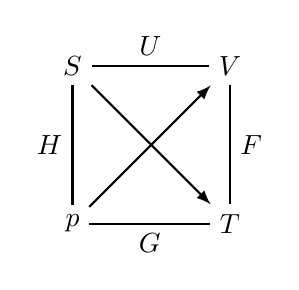
\begin{tikzpicture}
		\node(s)at(0,2){$S$};
		\node(v)at(2,2){$V$};
		\node(p)at(0,0){$p$};
		\node(t)at(2,0){$T$};
		\draw[thick](s)--(v)node[midway,above]{$U$};
		\draw[thick](s)--(p)node[midway,left]{$H$};
		\draw[thick](t)--(v)node[midway,right]{$F$};
		\draw[thick](t)--(p)node[midway,below]{$G$};
		\draw[thick,-latex](s)--(t);
		\draw[thick,-latex](p)--(v);
	\end{tikzpicture}
	\tikzchap Good physicists Have Studied Under Very Fine Teachers.
\end{center}
熵的标准全微分式:以$p,V,T$中两个为自变量,且将微分前系数用可测量表达出来的全微分式。比如以$T,V$
\[\d S=\kh{\pv ST}_V\d T+\kh{\pv SV}_T\d V=\frac{C_V}T\d T+\kh{\pv pT}_V\d V.\]
\paragraph*{附:偏导关系式}
微积分II中我们学过:
\begin{align}
	 & 1.       & \kh{\pv XY}_Z & =\kh{\pv YX}_Z^{-1};                                             \\
	 & 2.       & \kh{\pv XY}_Z & =\dvd{\kh{\pv XW}_Z}{\kh{\pv YW}_Z};  \\
	 & 3.^\star & \kh{\pv XY}_Z & =-\dvd{\kh{\pv ZY}_X}{\kh{\pv ZX}_Y}; \\
	 & 4.       & \kh{\pv XY}_Z & =\kh{\pv XY}_W+\kh{\pv XW}_Y\kh{\pv WY}_Z.
\end{align}
% 可以用Jaccobi行列式证明。

利用偏导关系式
\begin{align*}
	\kh{\pv ST}_p=\kh{\pv ST}_V+\kh{\pv SV}_T\kh{\pv VT}_p,
\end{align*}
由Maxwell关系
\[\kh{\pv SV}_T=\kh{\pv pT}_V=-\dvd{\kh{\pv VT}_p}{\kh{\pv Vp}_T}.\]
因此
\[C_p-C_V=-T\dvd{\kh{\pv VT}_p^2}{\kh{\pv Vp}_T}.\]

\paragraph*{响应函数}定义体膨张系数
\begin{align}
	\alpha:=\frac1V\kh{\pv VT}_p.
\end{align}
等温压缩系数
\begin{align}
	\kappa_T:=-\frac1V\kh{\pv Vp}_T.
\end{align}
可得
\begin{align}
	C_p-C_V=\frac{VT\alpha^2}{\kappa_T}\geqslant 0.
\end{align}
\begin{theorem}{热力学第三定律}{Third Law of Thermodynamics}
	% Nernst定理:
	$T\to 0$时,等温过程的熵变$\D_TS\to 0$

	Nernst原理:不可能使一个物体冷却到绝对温度的零度。
\end{theorem}

\clearpage
\section{复相系统的热力学性质}
复相系统:由几个物理性质均匀的部分构成,每一个均匀部分称为一相。特别的,化学成分相同,但相不同构成单元复项系统。
\subsection{粒子数可变系统的热力学方程}
开放系统粒子数可变,设均匀系有$k$个组元,粒子数分别为$N_1,\ldots,N_k$;描述系统时,除几何、力学参量外,需加上化学参量。

以$T,p,\hkh{N_i}$为自变量,适用Gibbs自由能,$G$是广延量
\[G(T,p,\lambda\hkh{N_i})=\lambda G(T,p,\hkh{N_i})\]
由
\begin{theorem}{Euler定理}{Euler's Theorem}
	若函数$f(x_1,\ldots,x_k)$满足$\forall\lambda\leqslant 0$
	\[f(\lambda x_1,\ldots,\lambda x_k)=\lambda^mf(x_1,\ldots,x_k).\]
	则可称为$m$阶齐次函数,且
	\[\sum_{i=1}^kx_i\pv f{x_i}=mf.\]
\end{theorem}
在两边对$\lambda$求导即可证明,继而
\[G=\sum_{i=1}^kN_i\kh{\pv G{N_i}}_{\neq N_i}=:\sum_{i=1}^kN_i\mu_i.\]
化学势$\mu_i$代表仅增加一个$i$组元粒子引起的$G$变化。摩尔Gibbs函数就是化学势$\mu$;孤立单元复相系,两相$\alpha$与$\beta$平衡的条件为化学势相同$\mu_\alpha=\mu_\beta$。
\paragraph*{化学反应}
考虑化学反应,设各化学计量数为$\nu_i$
\[0\rightleftharpoons\sum_{i=1}^r\nu_i{\mathrm A}_i.\]
在恒温恒压的条件下,平衡时Gibbs自由能%\footnote{在混合系统中,总势一般不是各组分简单相加。}
最小
\begin{align}
	\d G=\sum_{i=1}^r\mu_i\d N_i=\d n\cdot\sum_{i=1}^r\nu_i\mu_i=0.
\end{align}
应当注意:$\mu_i$均来自于混合系统的Gibbs自由能。

非平衡时,由$\vd G<0$,可得$\textstyle\sum\nu_i\mu_i>0$时,$\d n<0$,平衡逆向进行。
\iffalse
考虑一个由理想气体参与的化学反应,理想气体的化学势
\[\mu_i=RT\ln p_i+\cns(T).\]
带入上式可得,有
\[\sum_{i=1}^r\nu_iRT\ln p_i=\cns(T).\]
%\[\prod p_i^{\nu_i}=-\exp\kh{\sum\nu_i\phi_i}\]
又$p=RT\zkh{{\rm A}_i}$,%当$T$恒定时
\begin{align}
	\prod_{i=1}^r\zkh{{\rm A}_i}^{\nu_i}=:K(T).
\end{align}
%=(RT)^{-\sum\nu_i}\exp\kh{\sum\nu_i\phi_i}
$K$称为化学平衡常数,是$T$的函数。
\fi
\subsection{相变热力学}
前面已经提到,在有I和II两相共存的相变过程中,相变平衡的条件为$\mu_\mathrm I=\mu_\mathrm{II}$。

\paragraph*{Gibbs相律}有$n$个组分的系统在$r$个相共存时,系统$T,p,\mu_1,\ldots,\mu_n$共$(n+2)$个强度量,每个相有一个Gibbs-Duhem关系
\[S\d T-V\d p+\sum_{i=1}^nN_i\d\mu_i=0.\]
因此自由度
\begin{align}
	f=n+2-r.
\end{align}
\paragraph*{Clapeyron方程}
同种物质两相共存时化学势相同
\begin{center}
	\begin{tikzpicture}
		\coor44Tp;
		\draw[thick,domain=1:3]plot(\x,{e^\x/7+.5});
		\node at(1.5,2.5){II};
		\node at(3,1){I};
	\end{tikzpicture}
	\tikzchap   I为高温相,II为低温相
\end{center}
共存曲线下,
\[\mu_\mathrm I(T,p)=\mu_\mathrm{II}(T,p).\]
由$\d\mu=-s\d T+v\d p$
\iffalse
	故
	\[\pv{\mu_\mathrm I}T\d T+\pv{\mu_\mathrm I}p\d p=\pv{\mu_\mathrm{II}}T\d T+\pv{\mu_\mathrm{II}}p\d p.\]
	由Gibbs自由能给出Maxwell关系
	\begin{align*}
		\pw GTN=\pw GNT & \thus\kh{\pv\mu{T}}_N=-\kh{\pv SN}_T=-s, \\
		\pw GpN=\pw GNp & \thus\kh{\pv\mu{p}}_N=\kh{\pv VN}_p=v.
	\end{align*}
\fi
可得
\[\kh{s_\mathrm I-s_\mathrm{II}}\d T=\kh{v_\mathrm I-v_\mathrm{II}}\d p.\]
由I相转变II相中需要吸收的相变潜热
\[\ell:=T(s_\mathrm I-s_\mathrm{II}).\]
得到\textbf{Clapeyron方程}
\begin{align}
	\dv Tp=\frac{T(v_\mathrm I-v_\mathrm{II})}\ell.
\end{align}
该方程给出了凝固点或沸点随压强的变化。
\begin{center}
	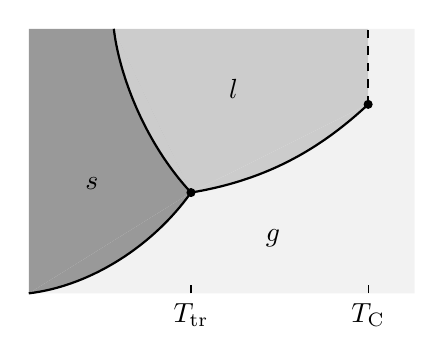
\begin{tikzpicture}
		\fill[gclr](0,0)--(2.06,1.28)--(4.31,2.4)--(4.31,3.36)--(4.9,3.36)--(4.9,0);
		\fill[sclr](0,0)--(2.06,1.28)--(1.08,3.36)--(0,3.36);
		\fill[lclr](2.06,1.28)--(1.08,3.36)--(4.31,3.36)--(4.31,2.4);
		%\shade[left color=lclr,right color=gclr](1.08,3.36) .. controls (1.14,2.83) and (1.44,1.95) .. (2.06,1.28)--(2.06,1.28) .. controls (3.03,1.44) and (3.71,1.84) .. (4.31,2.4)--(4.31,3.36);
		\draw[thick,fill=sclr](0,0) .. controls (0.76,0.09) and (1.56,0.58) .. (2.06,1.28) ;
		\draw[thick,fill=lclr](2.06,1.28) .. controls (3.03,1.44) and (3.71,1.84) .. (4.31,2.4) ;
		\draw[thick,fill=lclr](2.06,1.28) .. controls (1.44,1.95) and (1.14,2.83) .. (1.08,3.36) ;
		%\draw[dashed](2.06,1.28) .. controls (2.34,1.75) and (2.57,2.47) .. (2.64,3.35) ;
		\draw[dashed,thick](4.31,2.4)--(4.31,3.36);
		\draw[fill](2.06,1.28)circle(.05);
		\draw[fill](4.31,2.4)circle(.05);
		\coor{5.1}{3.6}Tp;
		\draw(2.06,0)node[below]{$T_\mathrm{tr}$}--(2.06,.1);
		\draw(4.31,0)node[below]{$T_\crt$}--(4.31,.1);
		\node at(.8,1.4){$\sfas$};
		\node at(3.1,.7){$\gfas$};
		\node at(2.6,2.6){$\lfas$};
	\end{tikzpicture}
	%\tikzchap 水的$T\vs p$图\\
	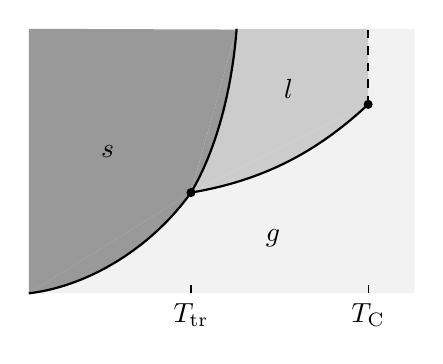
\begin{tikzpicture}
		\fill[gclr](0,0)--(2.06,1.28)--(4.31,2.4)--(4.31,3.36)--(4.9,3.36)--(4.9,0);
		\fill[sclr](0,0)--(2.06,1.28)--(2.64,3.35)--(0,3.36);
		\fill[lclr](2.06,1.28)--(2.64,3.36)--(4.31,3.36)--(4.31,2.4);
		\draw[thick,fill=sclr](0,0) .. controls (0.76,0.09) and (1.56,0.58) .. (2.06,1.28) ;
		\draw[thick,fill=lclr](2.06,1.28) .. controls (3.03,1.44) and (3.71,1.84) .. (4.31,2.4) ;
		%\draw[thick](2.06,1.28) .. controls (1.44,1.95) and (1.14,2.83) .. (1.08,3.36) ;
		\draw[thick,fill=sclr](2.06,1.28) .. controls (2.34,1.75) and (2.57,2.47) .. (2.64,3.36) ;
		\draw[dashed,thick](4.31,2.4)--(4.31,3.36);
		\draw[fill](2.06,1.28)circle(.05);
		\draw[fill](4.31,2.4)circle(.05);
		\coor{5.1}{3.6}Tp;
		\draw(2.06,0)node[below]{$T_\mathrm{tr}$}--(2.06,.1);
		\draw(4.31,0)node[below]{$T_\crt$}--(4.31,.1);
		\node at(1,1.8){$\sfas$};
		\node at(3.1,.7){$\gfas$};
		\node at(3.3,2.6){$\lfas$};
	\end{tikzpicture}
	\tikzchap 水(左)和一般纯净物(右)的$p\vs T$相图
\end{center}
对一般的汽-液相变,$v_\gfas\gg v_\lfas$,若气体符合理想气体,则有
\[\dv Tp\doteq\frac{Tv_\gfas}\ell=\frac{RT^2}{\ell p}\thus p=p_0\exp\fkh{\frac\ell{R}\kh{\frac1{T_0}-\frac1T}}.\]
水凝固存在反常膨胀,$\d T/\d p<0.$
\paragraph*{气液两相的转变和临界点}
考虑等温线
\begin{center}
	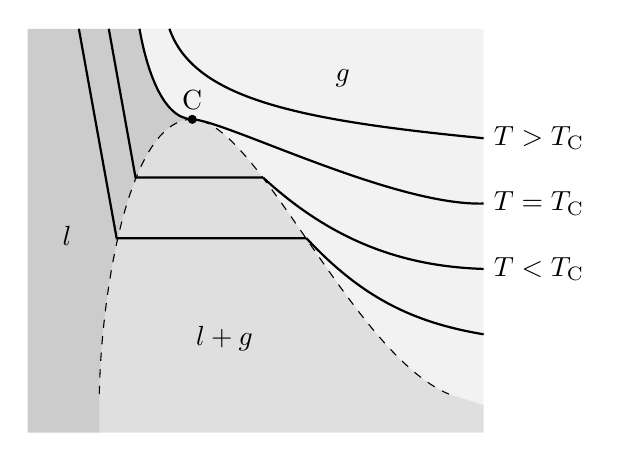
\begin{tikzpicture}
		\fill[lclr](0,0)--(0,5.13)--(1.42,5.13)--(2.09,3.98)--(0.91,0);
		\fill[gclr](1.42,5.13)--(2.09,3.98)--(3,.35)--(5.79,.35)--(5.79,5.13);
		\fill[glclr](0.91,0)--(0.91,.49)--(5.35,.49)--(5.79,0.35)--(5.79,0);
		\draw[dashed,fill=glclr](0.91,0.49) .. controls (0.93,1.72) and (1.27,3.98) .. (2.09,3.98) .. controls (2.91,3.98) and (4.11,1.01) .. (5.35,0.49) ;
		\draw[thick](0.65,5.13) -- (1.13,2.47) -- (3.54,2.47) ;
		\draw[thick](3.54,2.47) .. controls (4.24,1.72) and (4.89,1.4) .. (5.79,1.25) ;
		\draw[thick](1.03,5.13) -- (1.37,3.24) -- (2.99,3.24) ;
		\draw[thick](2.99,3.24) .. controls (3.9,2.4) and (4.82,2.11) .. (5.79,2.08)node[right]{$T<T_\crt$};
		\draw[thick,fill=gclr](1.42,5.13) .. controls (1.49,4.73) and (1.68,3.99) .. (2.09,3.98) .. controls (2.5,3.97) and (4.64,2.88) .. (5.79,2.91)node[right]{$T=T_\crt$};
		\draw[thick](1.8,5.13) .. controls (2.11,4.24) and (3.43,3.97) .. (5.79,3.74)node[right]{$T>T_\crt$};
		%\node[right]at(5.79,4.57){$T\gg T_\crt$};
		\coor6{5.5}Vp;
		\draw[fill](2.09,3.98)circle(.05)node[above]{C};
		\node at(.5,2.5){$\lfas$};
		\node at(2.5,1.2){$\lfas+\gfas$};
		\node at(4,4.5){$\gfas$};
	\end{tikzpicture}
	\tikzchap $p\vs V$相图,等温线
\end{center}
当$T<T_\crt$时,会存在气液共存区,在共存区中化学势相同
\[\mu_\lfas(T,p)=\mu_\gfas(T,p),\]
由于图中是等温线,所以共存区中等温线垂直于$p$轴;在临界点C有
\begin{align}
	\pv pV=0,\qquad\pv[2]pV=0.
\end{align}
理想气体不存在液化,下面考虑Van der Waals气体。
\begin{example}{Van der Waals气体的约化变量}{Reduced Variables of Van der Waals Gas}
	对于临界温度$T_\crt$
	\begin{align}
		\begin{cases}
			\pv pv=-\frac{RT}{(v-b)^2}+\frac{2a}{v^3}=0, \\
			\pv[2]pv=\frac{2RT}{(v-b)^3}-\frac{6a}{v^4}=0.
		\end{cases}\thus\begin{cases}
			v_\crt=3b,              \\
			T_\crt=\frac{8a}{27Rb}.
		\end{cases}.
	\end{align}
	此时
	\begin{align}
		p_\crt=\frac{RT_\crt}{v_\crt-b}-\frac a{v_\crt^2}=\frac a{27b^2}.
	\end{align}
	可以定义约化变量$\tilde T:=T/T_\crt$等,可得
	% \[\tilde p=\frac{8\tilde T}{3\tilde v-1}-\frac3{\tilde v^2}.\]
	\begin{align}
		\kh{\tilde p+\frac3{\tilde v^2}}\kh{\tilde v-\frac13}=\frac83\tilde T.
	\end{align}
\end{example}
气液共存线上气液摩尔比$x$,则
\[v=v_\gfas x+v_\lfas(1-x),\thus x=\frac{v-v_\lfas}{v_\gfas-v_\lfas}.\]
\begin{center}
	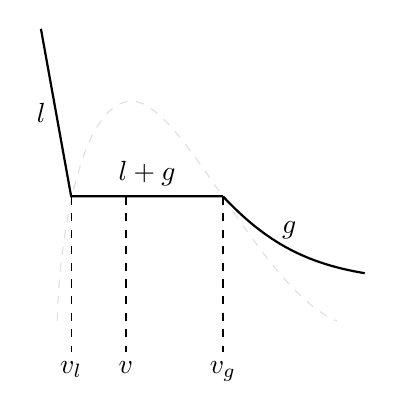
\begin{tikzpicture}[scale=.8]
		\draw[dashed,glclr](0.91,0.49) .. controls (0.93,1.72) and (1.27,3.98) .. (2.09,3.98) .. controls (2.91,3.98) and (4.11,1.01) .. (5.35,0.49) ;
		\draw[thick](0.65,5.13) -- (1.13,2.47)node[midway,left]{$\lfas$} -- (3.54,2.47)node[midway,above]{$\lfas+\gfas$};
		\draw[thick](3.54,2.47) .. controls (4.24,1.72) and (4.89,1.4) .. (5.79,1.25)node[midway,above]{$\gfas$};
		\coor6{5.5}vp;
		\draw[dashed](1.13,2.47)--(1.13,0)node[below]{$v_\lfas$};
		\draw[dashed](2,2.47)--(2,0)node[below]{$v$};
		\draw[dashed](3.54,2.47)--(3.54,0)node[below]{$v_\gfas$};
	\end{tikzpicture}
	\tikzchap 杠杆原理
\end{center}

投影到$T\vs V$图上与$p\vs V$图类似,只有$p<p_\crt$时才会有气液共存区,共存区的等压线垂直于$T$轴(对应沸点)。
\paragraph*{Landau相变理论}
在超导、磁性等一大类相变中,有一区别不同相的热力学量,称为序参量$\eta$。

无序相序参量$\eta=0$;有序相$\eta\neq 0$,对应对称破缺;$\eta$可以是复数(超导、超流);序参量有一维标量,也可以是二维和三维的。可以与
空间的维数不同。

相变中,Gibbs自由能
\[\d G=-S\d T-y\d Y+\sum\mu_i\d N_i=0,\]
对于固定$Y,T$下实现的过程有$\mu_i$必须相等,但对导数$S,y$无限制。若$S,y$在相变点不连续,则称相变为一级相变;若二阶导数不连续,则称为二级相变。

临界点:连续相变的相变点,临界温度$T_\crt$;临界现象:物质在连续相变临界点邻域的统计热力学行为。

唯象的,Landau自由能在临界点
\begin{align}
	F(T,\eta)=F_0(T)+\frac12a(T)\eta^2+\frac14b(T)\eta^4+\cdots,
\end{align}
由于系统对$\pm\eta$是对称的,展开中不含$\eta$的奇次幂。

求极值
\[\pv F\eta=\eta(a+b\eta^2)=0,\quad\pv[2]F\eta=a+3b\eta^2>0.\]
有三个解
\[\eta=0,\pm\sqrt{-\frac ab}.\]
$\eta=0$对应无序态,$T>T_\crt$;$\eta_\pm$对应有序态,$T<T_\crt$。当$T\to T_\crt$时,序参量$\eta$在$T_\crt$连续地由零转变到非零,即$a(T_\crt)=0$。

$T_\crt$附近泰勒展开
\[a(T)=a_0\kh{\frac T{T_\crt}-1},\quad b(T)=b_0.\]
$T<T_\crt$时,$a(T)<0$,故$b_0>0$。
\[\eta=\begin{cases}
	0,&T\geqslant T_\crt\\
	\pm\sqrt{\frac{a_0}{b_0}\kh{1-\frac T{T_\crt}}},&T<T_\crt
\end{cases}\]
临界指数$\beta=1/2$。

熵是连续的
\begin{align*}
	S=-\pv FT=S_0-\frac{a_0}{2T_\crt}\eta^2=
	\begin{cases}
		S_0,                             & T\geqslant T_\crt \\
		S_0+\frac{a_0^2}{2b_0T_\crt}\kh{\frac T{T_\crt}-1}, & T<T_\crt
	\end{cases}
	\rqed
\end{align*}
比热却不连续了,
\begin{align*}
	C=T\pv ST=
	\begin{cases}
		C_0,                 & T\geqslant T_\crt \\
		C_0+\frac{a_0^2}{2b_0T_\crt^2}T, & T<T_\crt
	\end{cases}
	\rqed
\end{align*}
因此是\textbf{二级相变}。有序相的比热大于无序相的比热,且$T=T_\crt$处比热的突变是有限的,$\alpha=\alpha'=1$。
\subparagraph*{外加场$B$}在弱场$B$下,序参量$m$
\[G(m,B)=F_0+\frac12am^2+\frac14bm^2-Bm.\]
平衡时
\[\pv Gm=a\eta+bm^3-B=0,\]
$T=T_\crt$时,$a=0,\;B=bm^3$故$\delta=3$。

磁化率
\[\chi=\mu_0\kh{\pv mB}_T=\frac{\mu_0}{a+3bm^3}=\begin{cases}
	\frac{\mu_0}{a_0}\kh{\frac T{T_\crt}-1}^{-1},&T\geqslant T_\crt \\
	\frac{\mu_0}{2a_0}\kh{\frac T{T_\crt}-1}^{-1}, & T<T_\crt
\end{cases}\]
$\gamma'=\gamma=1$。

临界指数$\alpha=1,\,\beta=1/2,\,\gamma=1,\,\delta=3$与实验结果有差异,原因是没考虑涨落。